As tecnologias de ambientes inteligentes est\~ao sendo desenvolvidas e ser\~ao um grande passo para as \'areas como constru\c{c}\~ao civil, industria, transporte e automa\c{c}\~ao residencial.

Para agirem de forma inteligente, estes ambientes necessitam de informa\c{c}\~ao sobre o contexto aonde ser\~ao implantados. As redes de sensores sem fio s\~ao um componente chave para estes ambientes, adquirem este contexto captando e comunicando os dados do ambiente \cite{lewis2004wireless}.

Este cap\'itulo apresenta uma vis\~ao geral sobre redes de sensores sem fio, arquitetura orientada a servi\c{c}os e os protocolos de aplica\c{c}ao existentes.

\section{Redes de sensores sem fio}

O desenvolvimento destas redes foi inicialmente motivada por aplica\c{c}\~oes militares e hoje s\~ao utilizados em diversas aplica\c{c}\~oes na ind\'ustria, no monitoramento e controle de processos industriais, supervis\~ao de maquinas, monitoramento de ambientes, estruturas e tubula\c{c}\~oes, automa\c{c}\~ao residencial, coleta de dados de pacientes, entre outros.

Avan\c{c}os recentes nas tecnologias de sistemas eletr\^onicos, semicondutores, sensores, microcontroladores e r\'adios tornaram poss\'ivel o desenvolvimento de redes de sensores de baixo custo e baixo consumo de energia uma realidade.

Os requisitos para uma rede de sensores distribu\'ida s\~ao: reconfigura\c{c}\~ao com esta\c{c}\~ao base, controle auton\^omo de opera\c{c}\~ao e ger\^encia de energia, auto-monitoramento, efici\^encia energ\'etica para longo tempo de opera\c{c}\~ao e apta a incorporar diversos sensores \cite{542724}.


Geralmente tais redes possuem centenas ou milhares de n\'os sensores e possuem as seguintes caracter\'isticas: pouca mem\'oria, pouco alcance do r\'adio, baixa capacidade de processamento e bateria, e custo reduzido. Comunicam-se entre si e com esta\c{c}\~oes base utilizando seus r\'adios sem fio, permitindo dissemina\c{c}\~ao da informa\c{c}\~ao para processamento remoto, visualiza\c{c}\~ao, an\'alise e armazenamento. A figura \ref{wsnOverview} d\'a uma vis\~ao geral sobre a comunica\c{c}\~ao destes n\'os.

\begin{figure}[H]
   \label{wsnOverview}
   \centering
   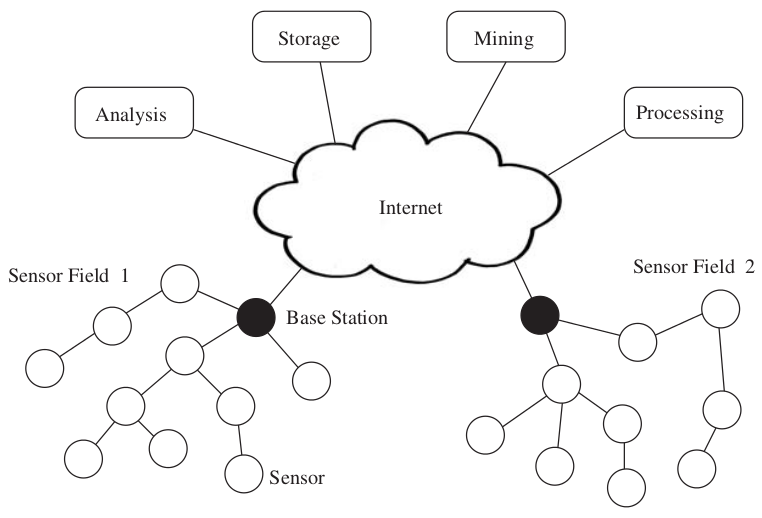
\includegraphics[width=0.8\textwidth]{figuras/wsn.png}
   \caption{Vis\~ao geral de uma RSSF \cite{dargie2010fundamentals}.}
\end{figure}

Um n\'o pertencente a esta rede geralmente \'e um dispositivo especificamente desenvolvido para um pr\'oposito, que possui poucos recursos computacionais e energ\'eticos e se comunicam entre seus semelhantes.

Muitas redes de sensores tamb\'em possuem atuadores, que permitem controle direto ao mundo real. Uma rede de sensores e atuadores recebe comandos da unidade de processamento (microcontrolador) e transforma estes comandos em sinais de entrada para um atuador, que interage com processos f\i'sicos. Estas redes s\~ao chamadas de redes de sensores e atuadores sem fio, ou WSAN.

A conserva\c{c}\~ao de energia \'e um dos objetivos das redes de sensores sem fio, pois n\~ao est\~ao ligados diretamente a fonte de energia. Deve-se minimizar o consumo em todos os n\'iveis do sistema, da aplica\c{c}\~ao at\'e o meio f\'isico, iniciando com o projeto de r\'adio. \cite{WsnSurvey2008} 

\subsection{N\'os sensores}
Sensores ligam o f\'isico com o mundo digital, capturando e revelando fen\^omenos do mundo real e convertendo em uma forma que pode ser processada, armazenada e utilizada para tomada de decis\~ao. A escolha entre qual sensor a ser utilizado depende muito da aplica\c{c}\~ao e da propriedade f\'isica a ser monitorada, alguns exemplos: temperatura, press\~ao, humidade, entre outros.

Geralmente os n\'o sensores s\~ao compostos por um microcontrolador, transceiver, mem\'oria externa, fonte de energia e um ou mais sensores. Os n\'os s\~ao respons\'aveis por coletar dados, fazer uma certa an\'alise da rede, correla\c{c}\~ao entre dados com outros n\'os e comunica\c{c}\~ao com uma esta\c{c}\~ao base afim de centralizar a informa\c{c}\~ao, para um processamento externo \cite{dargie2010fundamentals}.

\subsection{Sink Nodes}

Como estas redes utilizam um espectro diferente de comunica\c{c}\~ao, \'e necess\'ario uma integra\c{c}\~ao com a rede j\'a conhecida. Uma forma de integrar os n\'os sensores \'e utilizar n\'os espec\'ificos para executarem este trabalho.

Um exemplo \'e utilizar um n\'o como esta\c{c}\~ao de sincroniza\c{c}\~ao, por\'em surge um problema, pois o n\'o sincronizador deve ter conhecimento de todos os recursos dispon\'iveis na rede.

Quando os recursos s\~ao expostos diretamente pelo pr\'oprio dispositivo como num protocolo de aplica\c{c}\~ao tipo o CoAP a complexidade do n\'o gateway \'e bem reduzida, j\'a que o papel \'e simplesmente repassar os pacotes de descoberta de recursos para Internet \cite{Colitti11deintegrating}.


% descreva sobre as plataformas de \subsection{Plataforma de Hardware}
% descreva os \subsection{Sistema Operacional}
%
%\subsection{Rede de interconex\~ao}
%
%\subsection{Aplica\c{c}\~oes}

\section{Arquitetura orientada a servi\c{c}os}

Arquitetura orientada a servi\c{c}os \'e uma forma de organizar infraestrutura e aplica\c{c}\~oes de software em um conjunto de servi\c{c}os. Estes s\~ao oferecidos por prestadores de servi\c{c}o, servidores, organiza\c{c}\~oes que implementam os servi\c{c}os, fornecem descri\c{c}\~ao dos servic\c{c}os oferecidos, suporte t\'ecnico e de neg\'ocio.

O modelo de computa\c{c}\~ao utilizando este paradigma \'e conhecido como Computa\c{c}\~ao Orientada a servi\c{c}os (SOC) \cite{581580}.

Clientes destes servi\c{c}os podem ser outras solu\c{c}\~oes, aplica\c{c}\~oes, processos ou usu\'arios. Para satisfazer estes requisitos servi\c{c}os devem:
\begin{description}
    \item[Tecnologicamente neutros:] utilizar-se de padr\~oes reconhecidos e bem aceitos para comunica\c{c}\~ao, descri\c{c}\~ao e mecanismos de descoberta;
    \item[Baixo acoplamento:] detalhes desnecess\'arios (o qu\~ao desnecess\'ario precisa ser discutido) devem ser escondidos do cliente, que n\~ao precisa ter conhecimento sobre o funcionamento interno para utilizar o servi\c{c}o;
    \item[Localidade transparente:] clientes devem ser atendidos independentemente da localidade do servi\c{c}o dispon\'ivel.
\end{description}

SOA n\~ao \'e apenas uma arquitetura sobre servi\c{c}os, mas um relacionamento entre tr\^es entidades: o provedor de servi\c{c}o (service provider), descoberta de servi\c{c}o (service discovery agency) e o client (service requestor).  Abaixo a figura \ref{soaOverview} demonstra este relacionamento e suas intera\c{c}\~oes: publicar (publish), encontrar (find) e vincular (bind).

\begin{figure}[H]
   \label{soaOverview}
   \centering
   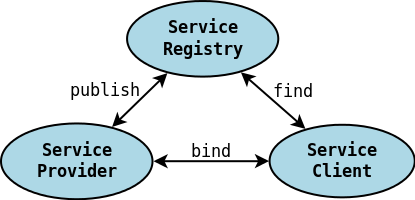
\includegraphics[width=0.6\textwidth]{figuras/soa.png}
   \caption{Arquitetura Orientada a Servi\c{c}os}
\end{figure}

%\section{REST}

\section{Webservices}

Um servi\c{c}o web \'e um sistema de software projetado para suportar interoperabilidade em intera\c{c}\~oes m\'aquina-a-m\'aquina na rede. Possui uma interface descritiva das funcionalidades num formato padronizado (especificamente WSDL). Esta nota\c{c}\~ao abstrata que deve ser implementada por um agente \cite{w3c-web-04}.

O agente \'e algo concreto, pode ser um peda\c{c}o de hardware ou software que recebe e envia mensagens. Um exemplo \'e implementar o mesmo servi\c{c}o web, utilizando agentes em diferentes linguagens. Embora o agente seja diferente, o servi\c{c}o Web continua o mesmo.

Servi\c{c}os Web prov\^em um padr\~ao para a interoperabilidade entre diferentes aplica\c{c}\~oes de software, que executam em diferentes plataformas de software e hardware.

\subsection{RESTful}

RESTFul \'e uma maneira de aplicar os princ\'ipios de design REST para servi\c{c}os web. Uma requisic\c{c}\~ao a um webservice RESTful, utiliza a informa\c{c}\~ao do m\'etodo como um verbo HTTP e a informa\c{c}\~ao do escopo ao qual o verbo ser\'a utilizado na URI. Ao contr\'ario um estilo RPC tende a ignorar o m\'etodo HTTP, procurando pelo m\'etodo a ser utilizado e o escopo na pr\'opria URI .

As opera\c{c}\~oes suportas s\~ao m\'etodos HTTP expl\'icitos que n\~ao salvam estado das aplica\c{c}\~oes clientes e s\~ao idempotentes, s\~ao eles:
\begin{description}
    \item[GET:] solicita ao webserver a representa\c{c}\~ao de uma informa\c{c}\~ao de um determinado recurso.
    \item[POST:] cria um recurso no webserver.
    \item[PUT:] muda o estado de um recurso do webserver.
    \item[DELETE:] remove o recurso ou alterar para um estado vazio.
\end{description}

Os Recursos usam um identificador \'unico e persistente, as URIs. A URIs possuem estruturas de diret\'orios, uma URI \'e uma \'arvore com ramos subordinados e superordinados conectando os n\'os \cite{rest}.


Para transfe\^encia de dados utiliza-se formatos gen\'ericos que enfatizam simplicidade e usabilidade pela internet, como XML e JSON. Resource Oriented Architecture \'e uma arquitetura boa para RESTful webservices \cite{richardson2008restful}.

Uma abordagem utilizando HTTP n\~ao \'e t\~ao interessante para uma aplica\c{c}\~ao de RSSF, j\'a que a quantidade de informa\c{c}\~ao a ser transmitida \'e consideravelmente maior. A figura \ref{bytesTransmitted} faz um comparativo entre o n\'umero de bytes transmitidos de diversos servidores web e seus protocolos.

\begin{figure}[H]
    \title{teste}
    \label{bytesTransmitted}
    \centering
    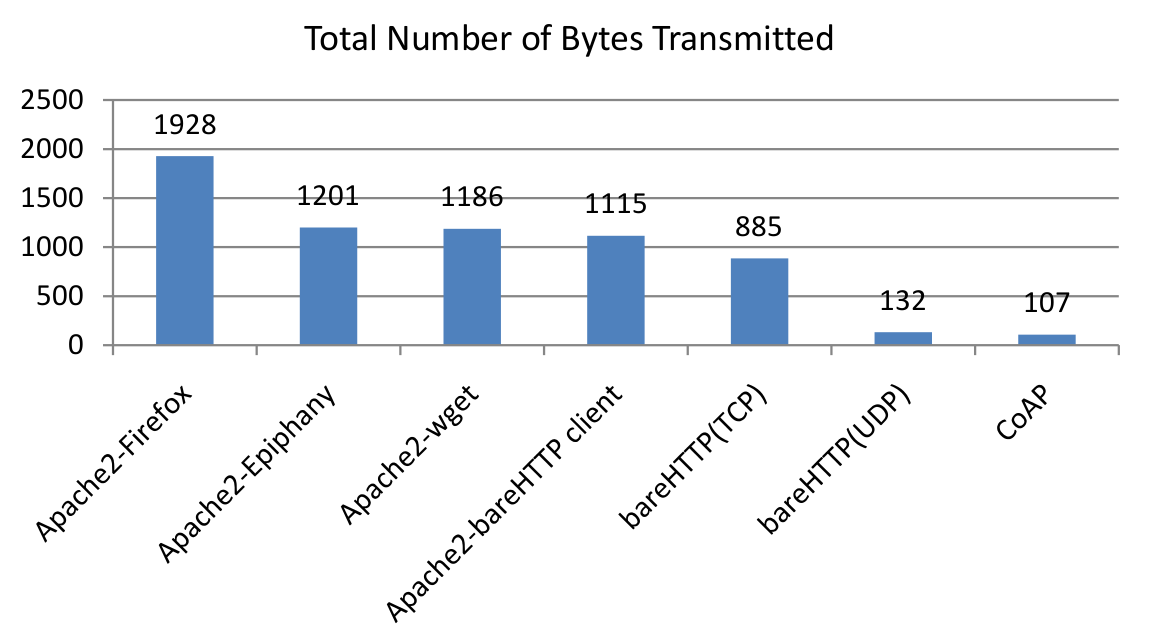
\includegraphics[width=0.9\textwidth]{figuras/bytestransmitted.png}
    \caption{Diferen\c{c}a de bytes transmitidos \cite{transportApp}.}
\end{figure}

Todos os webservices utilizam o conceito de URI, por\'em de maneiras diferentes. Mas um servi\c{c}o RESTful sempre exp\~oe a URI para cada peda\c{c}o de dado que o cliente quer operar sobre. Os principais competidores aos servi\c{c}os web RESTful s\~ao os RPC-styles.

%\section{Webservices em WSN}

\section{CoAP}

Um dos principais objetivos do CoAP \'e ser uma alternativa protocolo web gen\'erico para redes com dispositivos com restri\c{c}\~ao de energia e mem\'oria.

As vantagens de utilizar um protocolo compat\'ivel com o HTTP s\~ao a facilidade de integra\c{c}\~ao e o reuso de aplica\c{c}\~oes. CoAP \'e um conjunto REST otimizado para M2M, com suporte a descoberta de recursos, multicast e troca de mensagens ass\'incronas com simplicidade e baixo overhead.

A IETF estabelece as condi\c{c}\~oes m\'inimas para o desenvolvimento de um protocolo de aplica\c{c}\~ao compat\'ivel com HTTP, mas focado em aplica\c{c}\~oes aonde energia e mem\'oria s\~ao escassas. O protocolo CoAP foi projetado levando em considera\c{c}\~ao as restri\c{c}\~oes energ\'eticas e altas taxas de falha na transmiss\~ao dos pacotes em RSSF.

A comunica\c{c}\~ao entre os pontos no CoAP \'e ass\'incrona usando o UDP. A confiabilidade \'e um par\^ametro opcional e funciona atrav\'es de um mecanismo de retransmiss\~ao exponencial.

Possui 4 tipos de mensagem: Confirm\'avel, N\~ao-Confirm\'avel, Confirma\c{c}\~ao (ACK) e Reset. A figura \ref{coapFormat} mostra o formato do pacote.

\subsection{Formato das mensagens}
Uma mensagem CoAP deve caber num \'unico pacote IP, para que seja transmitida numa camada de enlace limitada.
\begin{figure}[H]
    \label{coapFormat}
    \centering
    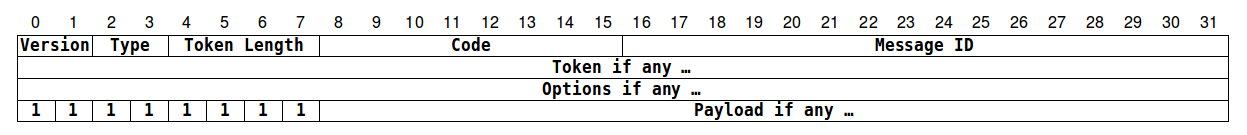
\includegraphics[width=0.6\textwidth]{figuras/formato.png}
    \caption{Formato do pacote CoAP  em bits \cite{draft-ietf-core-coap-18}.}
\end{figure}


Os campos do pacote CoAP s\~ao: a vers\~ao do CoAP, implementa\c{c}\~oes devem utilizar este campo com o valor 1. O tipo: campo para definir o tipo da mensagem: Confirm\'avel (0), N\~ao-Confirm\'avel (1) , de Confirma\c{c}\~ao (2) ou Reset (3).

O tamanho do Token: utilizado para controle de requisi\c{c}\~oes e repostas. O tamanho do Token pode variar entre 0 e 8 bytes. Tamanhos entre 9 a 15 s\~ao reservados e n\~ao devem ser usados. \'E um campo sempre gerado pelo cliente CoAP.

O C\'odigo: separados em 3-bit mais significativos para classes e 5-bits menos significativos para detalhe. As classes podem indicar uma requisi\c{c}\~ao (0), uma resposta de sucesso (2), e uma resposta de erro do cliente (4), ou uma resposta de erro do servidor (5), as outras classes s\~ao reservadas. Em um caso especial o c\'odigo 0.00 indica uma mensagem vazia.

O ID da mensagem: usada para deduplica\c{c}\~ao de mensagens e confirma\c{c}\~ao ou reset de mensagens. \'E gerado por quem envia a mensagem, no caso de uma mensagem confirm\'avel ou reset, a resposta deve possuir o ID da mensagem enviada. A implemeta\c{c}\~ao da gera\c{c}\~ao dos IDs est\'a aberta, depende da aplica\c{c}\~ao que o CoAP ser\'a usado, por\'em \'e recomendado que o valor inicial seja rand\^omico.
   
%Codifica\c{c}\~ao das op\c{c}\~oes
\subsection{Transmiss\~ao de Mensagens}
A transmiss\~ao de mensagems \'e controlada basicamente pelos par\^ametros: ACK TIMEOUT, ACK RANDOM FACTOR, MAX RETRANSMIT, NSTART, Leisure e PROBING RATE.

Estes par\^ametros s\~ao respectivamente: o tempo que uma mensagem confirm\'avel aguarda o ACK; fator de randomicidade para gerar os ACK TIMEOUTs subsequentes; contador para o n\'umero m\'aximo de tentativas de retransmiss\~ao; n\'umero limite de intera\c{c}\~oes simult\^aneas mantidas por um servidor.

A Leisure \'e o tempo que o servidor aguarda para responder uma requisi\c{c}\~ao multicast, \'e calculada: $Leisure = S * G / R$. Aonde S \'e o tamanho estimado da reposta, G \'e uma estimativa do tamanho do grupo e R \'e a taxa de transmiss\~ao. PROBING RATE: \'e a taxa m\'edia para transmiss\~ao de dados.

    Estes par\^ametros definem a temporiza\c{c}\~ao do sistema. Os valores padr\~oes s\~ao mostrados na Tabela \ref{coapDefault}.
\begin{table}[h]
\label{coapDefault}
\centering
\begin{tabular}{@{}lllll@{}}
\toprule
Nome & Valor padr\~ao & \\ \midrule
ACK timeout & 2 segundos & \\
ACK random factor & 1.5 & \\
NStart & 1 & \\
Default Leisure & 5 segundos & \\
Probing rate & 1 Byte/segundo & \\
Max retransmit & 4 &  \\ \midrule
\end{tabular}
\caption{Valores padr\~ao do CoAP.}
\end{table}

A retransmiss\~ao \'e controlada por um timeout e um contador. Inicialmente o contador \'e zero e atribuido um valor rand\^omico entre o ACK TIMEOUT e (ACK RANDOM FACTOR * ACK TIMEOUT) para o timeout. Quando este timeout \'e atigido o contador \'e incrementado e o timeout duplicado.

Uma falha na transmiss\~ao ocorre quando atingir o n\'umero m\'aximo de tentavivas ou receber uma mensagem de RESET. Quando receber um ACK a transmiss\~ao da mensagem confirm\'avel \'e completa. O servidor ir\'a ignorar mensagens que chegam por multicast quando n\~ao puder responder nada de \'util.

Na situa\c{c}\~ao aonde possuir uma informa\c{c}\~ao suficientemente nova pode responder na pr\'opria mensagem de confirma\c{c}\~ao (ACK). Essa t\'ecnica \'e chamada de ''Piggy-backed'' um mecanismo de transmiss\~ao para mensagens confirmadas, o cen\'ario \'e ilustrado na Figura \ref{piggyBacked}\cite{draft-ietf-core-coap-18}.
\begin{figure}[H]
   \label{piggyBacked}
   \centering
   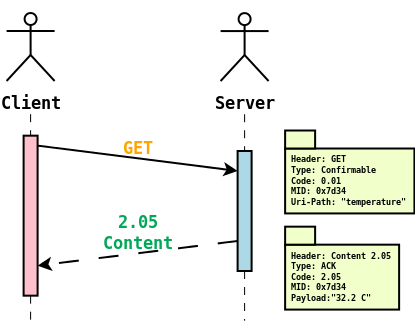
\includegraphics[width=0.6\textwidth]{figuras/piggybacked.png}
   \caption{Resposta na mensagem de confirma\c{c}\~ao, chamado de piggy-backed.}
\end{figure}

\subsection{Requisi\c{c}\~ao e Resposta}

Uma requisi\c{c}\~ao \'e inicializada ao preencher o campo c\'odigo no cabe\c{c}alho do CoAP e gerar um token.
Para finalizar o fluxo \'e necess\'ario que a resposta chegue e o token seja o mesmo.

Fluxo esperado de requisi\c{c}\~ao sem confirma\c{c}\~ao na figura \ref{nonConfirmable}.
\begin{figure}[H]
   \label{nonConfirmable}
   \centering
   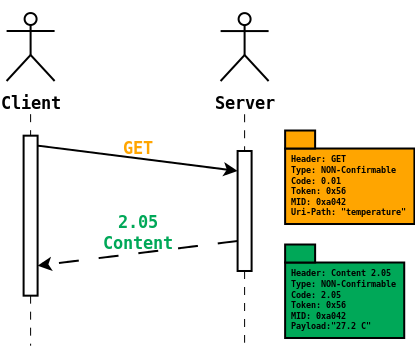
\includegraphics[width=0.6\textwidth]{figuras/nonconfirmable.png}
   \caption{Fluxo esperado de requisi\c{c}\~ao e resposta sem confirma\c{c}\~ao}
\end{figure}

A especifica\c{c}\~ao tamb\'em prev\^e fluxo de requisi\c{c}\~ao com confirma\c{c}\~ao, e resposta separada com confirma\c{c}\~ao. A figura \ref{separateResponse} exemplifica:

\begin{figure}[H]
   \label{separateResponse}
   \centering
   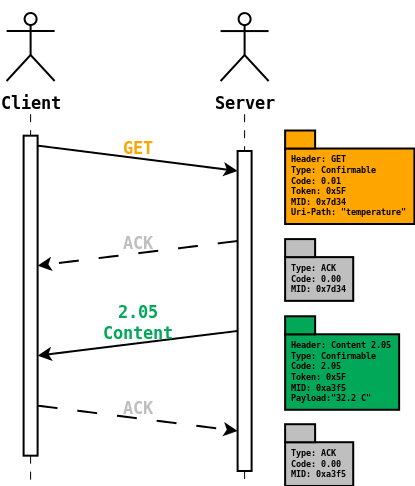
\includegraphics[width=0.6\textwidth]{figuras/separateresponse.png}
   \caption{Fluxo esperado de requisi\c{c}\~ao e resposta com confirma\c{c}\~ao, com resposta separada}
\end{figure}

A descoberta de recursos \'e feita quando um servidor recebe uma requisi\c{c}\~ao GET para o recurso ~/well-know/core. O servidor CoAP deve responder no formato CORE link Format\cite{rfc6690}. A descoberta de servi\c{c}os no protocolo CoAP \'e feita atrav\'es de socket Multicast. Os recursos s\~ao identificados por uma URI, e os m\'etodos s\~ao implementados de forma similar ao HTTP.  
\section{EPOS}
O EPOS \'e um sistema operacional multithread com suporte a preemp\c{c}\~ao, desenvolvido em C++ que faz uso intenso de programa\c{c}\~ao orientada a aspectos utilizando templates.

Foi projetado utilizando ADESD, Application Driven Embedded System Design, um m\'etodo para projeto de sistemas embarcados orientados \`a aplica\c{c}\~ao. Esta metodologia guia o desenvolvimento paralelo de hardware e software al\'em de manter portabilidade. O EPOS possui porte para as seguintes arquiteturas: MIPS, IA32, PowerPC, H8, Sparc, AVR e ARM. \cite{eposProject}

A portabilidade \'e atingida utilizando entidades chamadas de Mediadores de Hardware que fornecem interfaces simples para acesso as fun\c{c}\~oes espec\'ificas de arquitetura. Estas interfaces s\~ao utilizadas por entidades abstratas como alarmes e threads peri\'odicas. Abaixo uma a figura \ref{eposOverview} ilustrando a vis\~ao geral do EPOS.

\begin{figure}[H]
   \label{eposOverview}
   \centering
   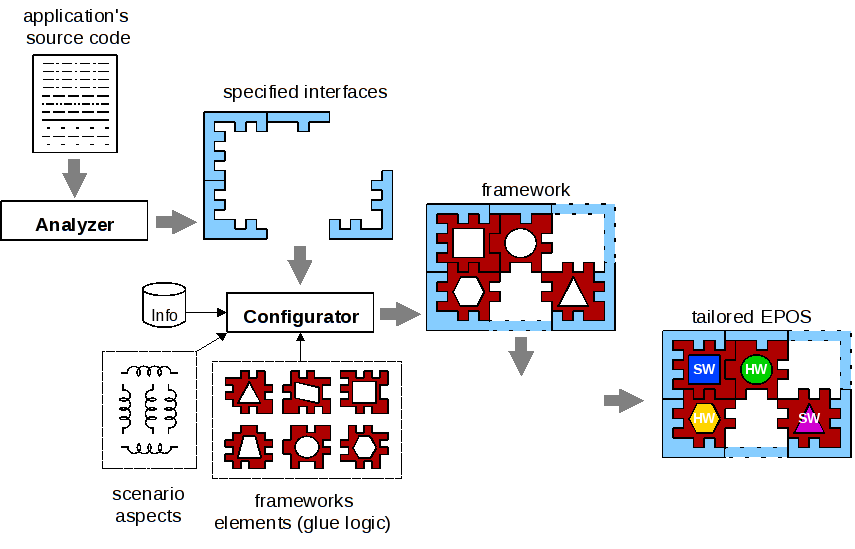
\includegraphics[width=0.8\textwidth]{figuras/eposOverview.png}
   \caption{Overview do EPOS.}
\end{figure}

 
O EPOS tamb\'em possui uma interface de software/hardware que abstrai sensores de forma uniforme, definindo classes de dispositivos baseados numa finalidade. Possui abstra\c{c}\~oes para entidades temporais como rel\'ogio, alarme e cron\^ometro, biblioteca com estruturas de dados e sequenciadores. Permitindo o uso de ferramentas para gera\c{c}\~ao automatizada de abstra\c{c}\~oes de sistemas \cite{epos}.

A infraestrutura de comunicaca\c{c}\~ao do EPOS para redes de sensores sem-fio \'e implementada pelo protocolo C-MAC, Configurable MAC, que prov\^e suporte a comunicaca\c{c}\~ao de baixo n\'ivel (MAC - Medium Access Control).

Possui uma pilha de protocolos basedo na arquitetura OSI e outra abordagem Cross-layer. A implementa\c{c}\~ao IPv4 utiliza um controle de fluxo aonde os n\'os sinalizam a disponibilidade de buffer para mensagem \'unica em tempos ajustando o tempo entre a troca de mensagens \cite{eposCrossLayer}.


\section{Trabalhos Relacionados}

\subsection{OpenWSN}

O projeto OpenWSN \'e um projeto de redes de sensores sem fio de c\'odigo aberto que confia na comunidade para manter atualizado e encontrar erros. Possui uma implementa\c{c}\~ao completa de c\'odigo aberto, das pilhas de protocolos padr\~oes pra Internet das Coisas. O OpenWSN tamb\'em possu\'i a primeira implementa\c{c}\~ao aberta do padr\~ao 802.15.4e, Time Synchronized Channel Hopping.

Por serem sincronizados os motes precisam acordar apenas para transmitir ou receber e periodicamente se comunicar para manter a rede sincronizada quando estiver inativo. Este overhead de temporiza\c{c}\~ao \'e pequeno, cerca de 0.02\% de ciclo de trabalho do r\'adio \cite{openWSNPaper}.

A pilha de protocolos \'e totalmente implementada em C e pode ser compilada em qualquer toolchain que suporte uma plataforma alvo. Possui porte para diversas plataformas de microcontroladores de 16 bits e para as arquiteturas mais novas de 32 bits dos Cortex-M. O projeto possui diversas ferramentas para depura\c{c}\~ao, simula\c{c}\~ao e ambiente necess\'ario para integrar as aplica\c{c}\~oes a Internet \cite{openWSN}.

Resultados experimentais de uma rede de motes demonstram que os r\'adios operam num ciclo m\'edio de trabalho de $0.1\%$ e uma m\'edia de 0.68 $\mu$A em hardware comum. Este consumo baixo permite uma vasta gama de aplica\c{c}\~oes.

\subsection{Contiki}
O Contiki \'e um sistema operacional criado por Adam Dunkels em 2000, escrito em C, de c\'odigo aberto para sistemas com restri\c{c}\~ao de recursos comunicarem numa rede. Foi desenvolvido para ser um sistema operacional para Internet das coisas. Possui uma camada de abstra\c{c}\~ao RESTful para web services chamada Erbium, que implementa o protocolo CoAP.

Cada processo no Contiki possui bloco de controle, que cont\'em informa\-\c{c}\~oes de tempo de execu\c{c}\~ao do processo e uma refer\^encia para uma protothread, na qual o c\'ogido \'e armazenado na ROM. 

Programas s\~ao escritos num modelo dirigido a eventos, geralmente s\~ao implementados como m\'aquinas de estados expl\'icitos, que com um grande n\'umero de estados o c\'odigo come\c{c}a a se tornar complexo, dif\'icil de entender e depurar. Estas foram as principais motiva\c{c}\~oes para que fosse desenvolvido um modelo de programa\c{c}\~ao diferente, utilizado nos projetos desenvolvidos por Dunkels, a pilha uIP e do Contiki \cite{Dunkels05protothreads}.

O conceito protothread foi desenvolvido por Adam Dunkels em 2005, uma combina\c{c}\~ao entre eventos e threads, possuem comportamentos de bloqueio e espera, que permite o intersequenciamento dos eventos, gerando um baixo overhead de mem\'oria por n\~ao necessitar de salvamento de contexto. Foi desenvolvida para diminuir a complexidade de c\'odigo 

As limita\c{c}\~oes dessas t\'ecnicas s\~ao: vari\'aveis autom\'aticas n\~ao s\~ao preservadas Stack durante trocas de contexto entre as protothreads. Elas podem ser utilizadas durante uma protothread mas devem ser salvas antes da execu\c{c}\~ao de do m\'etodo WAITING. Al\'em disso programas que utilizam protothreads n\~ao podem utilizar switch case, caso o fizer um erro de compila\c{c}\~ao \'e esperado.

Cada protothread consome 2 bytes de mem\'oria, que s\~ao utilizados para armazenar a continuidade local, uma referencia utilizada em um pulo condicional durante a execu\c{c}\~ao da thread. \'E um m\'etodo similar ao mecanismo de Duffy e Co-rotina em C \cite{duffyMechanism}.

O Contiki prop\~oe uma estrat\'egia de ciclos de trabalho que consegue manter um n\'o comunic\'avel em uma rede, por\'em com seus r\'adios desligados em aproximadamente 99\% do tempo \cite{Dunkels11thecontikimac}.

\subsection{LibCoap}
LibCoap \'e uma biblioteca implementada em C do protocolo CoAP. Possui 292K de tamanho compilada estaticamente em sua vers\~ao 4.0.1.
A licensa da biblioteca \'e GPL (2 ou maior) ou licensa BSD revisada.

Possui uma su\'ite de testes para regress\~ao, utilizando o framework de testes CUnit (http://cunit.sourceforge.net/). A documenta\c{c}\~ao pode ser encontrada em: http://libcoap.sourceforge.net/.

\'E uma biblioteca auto-condida, que possui parser do protocolo e fun\c{c}\~oes b\'asicas de rede. Depende de implementa\c{c}\~ao de sockets tipo BSD e malloc. Possui implementa\c{c}\~ao de Hash, String e URI utilizados para montar os pacotes CoAP.

Possui um m\'odulo de rede, aonde \'e implementado as fun\c{c}\~oes de envio/recebimento de requisi\c{c}\~oes e respostas, com confirma\c{c}\~ao, sem confirma\c{c}\~ao, mensagem de reset e erros.

\'E poss\'ivel selecionar a camada de transporte \'e necess\'ario selecionar utilizando flags de preprocessamento. O padr\~ao \'e socket POSIX. A pilha uIP \'e selecionada com a flag -DWITH\textunderscore CONTIKI, ou para selecionar a pilha lwIP -DWITH\textunderscore LWIP.

\subsection{CantCoap}
\'E uma implementa\c{c}\~ao em C++ desenvolvida por Ashley Mills em 2013. Esta biblioteca foca na simplicidade e oferece um conjuto m\'inimo para montar pacotes CoAP.

Tamb\'em \'e poss\'ivel montar os pacotes CoAP a partir de uma sequ\^encia de caracteres recebidos de uma placa de rede. Abaixo exemplos de uso da biblioteca retirados de https://github.com/staropram/cantcoap.

\lstdefinestyle{customc}{
  belowcaptionskip=1\baselineskip,
  breaklines=true,
  xleftmargin=\parindent,
  language=C++,
  showstringspaces=false,
  basicstyle=\scriptsize\ttfamily,
  keywordstyle=\bfseries\color{black},
  commentstyle=\itshape\color{blue},
  identifierstyle=\color{black},
  stringstyle=\color{red},
}

\lstset{escapechar=@,style=customc}

Abaixo um exemplo de uso para montar um pacote e enviar:

\begin{lstlisting}
CoapPDU *pdu = new CoapPDU();
pdu->setType(CoapPDU::COAP_CONFIRMABLE);
pdu->setCode(CoapPDU::COAP_GET);
pdu->setToken((uint8_t*)"\3\2\1\0",4);
pdu->setMessageID(0x0005);
pdu->setURI((char*)"test",4);

/* send packet */
ret = send(sockfd,pdu->getPDUPointer(),pdu->getPDULength(),0);
\end{lstlisting}

Quando receber a mensagem a forma de uso \'e mostrada abaixo:
\begin{lstlisting}
// receive packet
ret = recvfrom(sockfd,&buffer,BUF_LEN,0,recvAddr,recvAddrLen);
CoapPDU *recvPDU = new CoapPDU((uint8_t*)buffer,ret);
if(recvPDU->validate()) {
    recvPDU->getURI(uriBuffer,URI_BUF_LEN,&recvURILen);
    ...
}
\end{lstlisting}

Por ser uma biblioteca bem simplificada e n\~ao possuir depend\^encias diretas com a implementa\c{c}\~ao da camada de transporte e ser c\'odigo livre, foi escolhida como base para a implementa\c{c}\~ao teste do trabalho.
